\begin{enumerate}

    \item-
    \\
    \textbf{Solución item C:}
    \begin{verbatim}
       var_mues      P(s^2)
        0.00         0.42
        0.50         0.48
        2.00         0.10
    \end{verbatim}
    
    \begin{lstlisting}[frame=single]
    x <- c(0, 0.5, 2)
    p <- c(0.42, 0.48, 0.10)
    df2 <- data.frame(x, p)
    library(tidyverse)
    ggplot(df2, aes(x, p))+geom_bar(stat="identity",width=0.25)
    \end{lstlisting}
    
    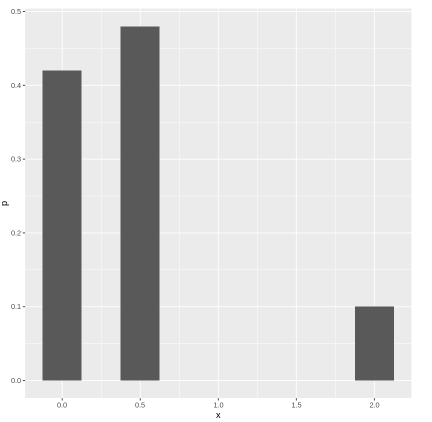
\includegraphics[scale=0.8]{img/v_muest.png}
    
    \textbf{Solución item D:}
    $$
    \mu_ {\bar{x}} =E[\bar{X}]=\sum_{i}^{}\bar{x}*P(\bar{X}=\bar{x_i})\\$$$$
    =(1)*0.25+(1.5)*0.4+(2)*0.26+(2.5)*0.08+(3)*0.01\\$$$$
    =1.6\\\\$$$$
    $$
    $$
    \sigma_ {\bar{x}}^2 =E[(\bar{X}-E[\bar{X}])^2]=\sum_{i}^{}(\bar{x_i}-1.6)^2*P(\bar{X}=\bar{x_i})\\$$$$
    =(1-1.6)^2*0.25+ . . . + (3-1.6)^2*0.01\\$$$$
    =0.22
    $$

\end{enumerate}